\documentclass[tikz,border=12pt]{standalone}
\usepackage{circuitikz}
\usepackage{xcolor}
\usepackage{amsmath}
\usepackage{amssymb}
\usetikzlibrary{arrows.meta, positioning, decorations.pathreplacing, calc, fit, backgrounds}

\begin{document}
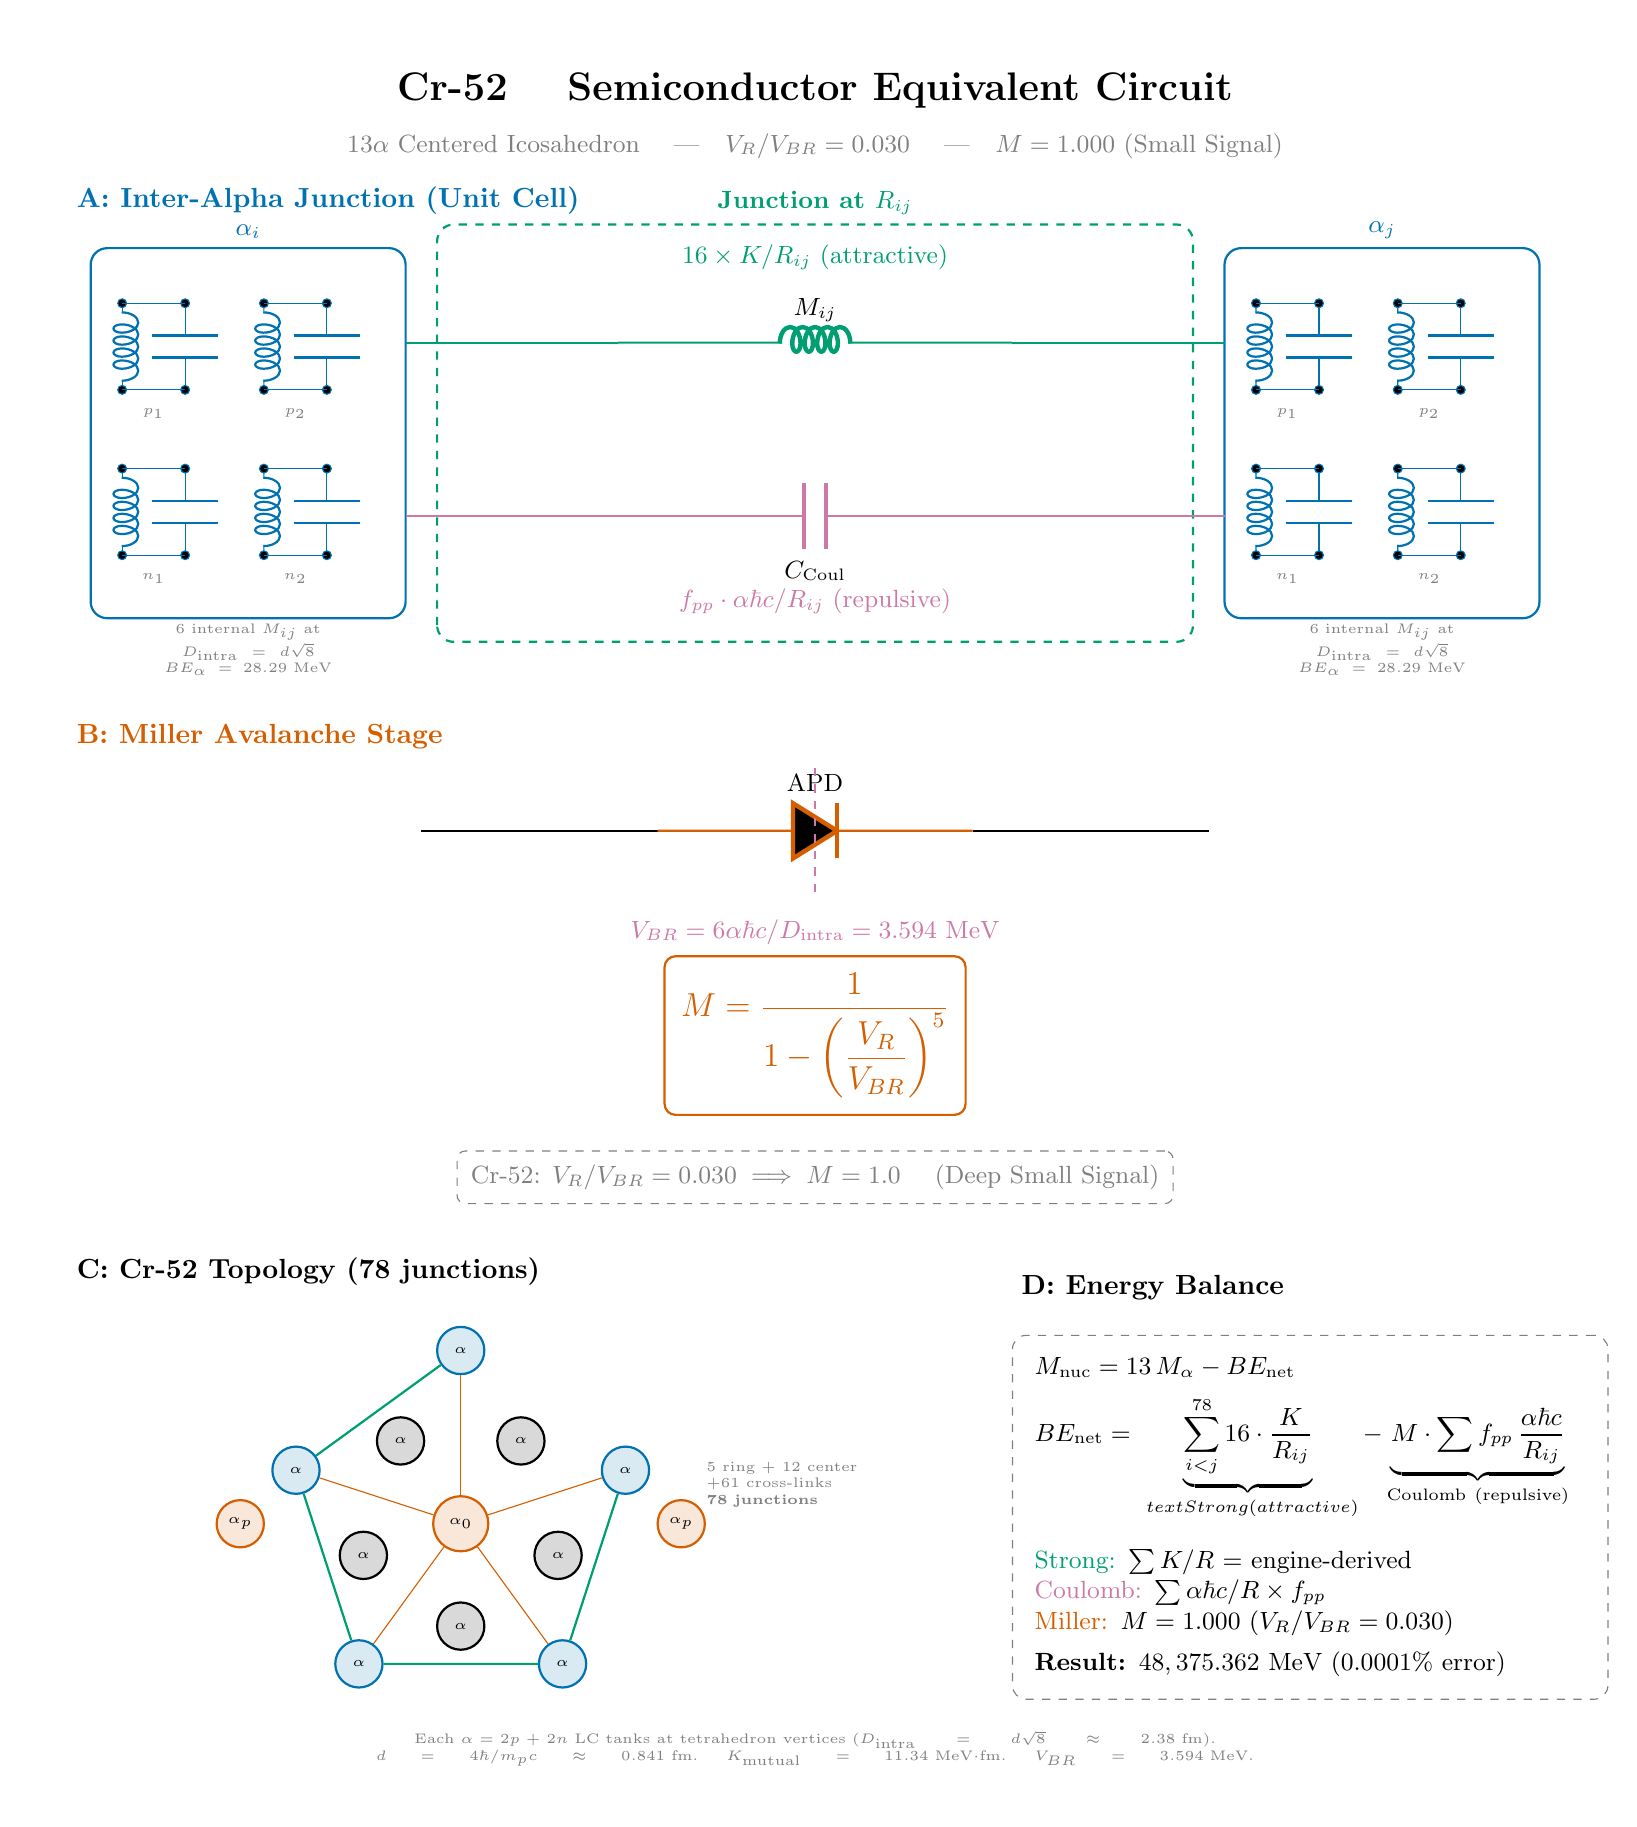
\begin{tikzpicture}[>=latex, font=\small]

% --- AVE house figure style: WHITE print profile, Okabe-Ito colourblind-safe palette.
%     Single source of truth: src/ave/viz/README.md + src/ave/viz/style.py. `ave.viz` is
%     matplotlib-only (it has no TikZ mechanism), so the hex values below are copied BY HAND
%     from style.py -- COLORS (the semantic dict) and _PROP_CYCLE (the extended Okabe-Ito set).
%     Re-derive from style.py, do not re-tune here. Every colour below clears 3:1 contrast on
%     white; the retired neon set was defined against a 15/15/15 base and measures 1.3-2.0:1
%     on white (i.e. it would ship as mud, not as colour).
\definecolor{aveblue}{HTML}{0072B2}       % COLORS["ave"]        -- alpha-cluster LC tanks
\definecolor{aveaccent}{HTML}{009E73}     % COLORS["accent"]     -- mutual-inductance bus (strong/attractive)
\definecolor{avevermillion}{HTML}{D55E00} % COLORS["comparison"] -- Miller avalanche / halo channel
\definecolor{avepurple}{HTML}{CC79A7}     % _PROP_CYCLE reddish-purple -- Coulomb repulsion
\definecolor{aveink}{HTML}{000000}        % COLORS["data"]       -- polar alpha caps + body text
\definecolor{avemuted}{HTML}{7F7F7F}      % COLORS["muted"]      -- annotations, dashed frames

% Background: WHITE (house print profile). The prior `\fill[darkbg] (-10,-13.5) rectangle
% (10,9)` canvas is REMOVED rather than recoloured, per the ratified circuit_h3_decay restyle.
% It is replaced by an unpainted `\path` over the SAME rectangle so the standalone bounding
% box -- and therefore every figure's page size and aspect ratio in the manuscript -- is
% preserved exactly. Dropping the rectangle outright would shrink-wrap the bbox and silently
% re-scale every \includegraphics that carries these figures.
\path (-10,-13.5) rectangle (10,9);

% TITLE
\node[text=aveink, font=\bfseries\Large] at (0, 8.2)
    {Cr-52 \quad Semiconductor Equivalent Circuit};
\node[text=avemuted, font=\small] at (0, 7.5)
    {$13\alpha$ Centered Icosahedron \quad|\quad $V_R/V_{BR} = 0.030$ \quad|\quad $M = 1.000$ (Small Signal)};

% =====================================================================
% SECTION A: INTER-ALPHA JUNCTION (UNIT CELL)
% =====================================================================

\node[text=aveblue, font=\bfseries, anchor=west] at (-9.5, 6.8) {A: Inter-Alpha Junction (Unit Cell)};

% --- LEFT ALPHA ---
\draw[aveblue, thick, rounded corners=6pt] (-9.2, 1.5) rectangle (-5.2, 6.2);
\node[text=aveblue, font=\bfseries\small, anchor=south] at (-7.2, 6.2) {$\alpha_i$};

\draw[aveblue] (-8.8, 5.5) to[L, *-*] (-8.8, 4.4);
\draw[aveblue] (-8.0, 5.5) to[C, *-*] (-8.0, 4.4);
\draw[aveblue] (-8.8, 5.5) -- (-8.0, 5.5); \draw[aveblue] (-8.8, 4.4) -- (-8.0, 4.4);
\node[text=avemuted, font=\tiny] at (-8.4, 4.1) {$p_1$};

\draw[aveblue] (-7.0, 5.5) to[L, *-*] (-7.0, 4.4);
\draw[aveblue] (-6.2, 5.5) to[C, *-*] (-6.2, 4.4);
\draw[aveblue] (-7.0, 5.5) -- (-6.2, 5.5); \draw[aveblue] (-7.0, 4.4) -- (-6.2, 4.4);
\node[text=avemuted, font=\tiny] at (-6.6, 4.1) {$p_2$};

\draw[aveblue] (-8.8, 3.4) to[L, *-*] (-8.8, 2.3);
\draw[aveblue] (-8.0, 3.4) to[C, *-*] (-8.0, 2.3);
\draw[aveblue] (-8.8, 3.4) -- (-8.0, 3.4); \draw[aveblue] (-8.8, 2.3) -- (-8.0, 2.3);
\node[text=avemuted, font=\tiny] at (-8.4, 2.0) {$n_1$};

\draw[aveblue] (-7.0, 3.4) to[L, *-*] (-7.0, 2.3);
\draw[aveblue] (-6.2, 3.4) to[C, *-*] (-6.2, 2.3);
\draw[aveblue] (-7.0, 3.4) -- (-6.2, 3.4); \draw[aveblue] (-7.0, 2.3) -- (-6.2, 2.3);
\node[text=avemuted, font=\tiny] at (-6.6, 2.0) {$n_2$};

% --- RIGHT ALPHA ---
\draw[aveblue, thick, rounded corners=6pt] (5.2, 1.5) rectangle (9.2, 6.2);
\node[text=aveblue, font=\bfseries\small, anchor=south] at (7.2, 6.2) {$\alpha_j$};

\draw[aveblue] (5.6, 5.5) to[L, *-*] (5.6, 4.4);
\draw[aveblue] (6.4, 5.5) to[C, *-*] (6.4, 4.4);
\draw[aveblue] (5.6, 5.5) -- (6.4, 5.5); \draw[aveblue] (5.6, 4.4) -- (6.4, 4.4);
\node[text=avemuted, font=\tiny] at (6.0, 4.1) {$p_1$};

\draw[aveblue] (7.4, 5.5) to[L, *-*] (7.4, 4.4);
\draw[aveblue] (8.2, 5.5) to[C, *-*] (8.2, 4.4);
\draw[aveblue] (7.4, 5.5) -- (8.2, 5.5); \draw[aveblue] (7.4, 4.4) -- (8.2, 4.4);
\node[text=avemuted, font=\tiny] at (7.8, 4.1) {$p_2$};

\draw[aveblue] (5.6, 3.4) to[L, *-*] (5.6, 2.3);
\draw[aveblue] (6.4, 3.4) to[C, *-*] (6.4, 2.3);
\draw[aveblue] (5.6, 3.4) -- (6.4, 3.4); \draw[aveblue] (5.6, 2.3) -- (6.4, 2.3);
\node[text=avemuted, font=\tiny] at (6.0, 2.0) {$n_1$};

\draw[aveblue] (7.4, 3.4) to[L, *-*] (7.4, 2.3);
\draw[aveblue] (8.2, 3.4) to[C, *-*] (8.2, 2.3);
\draw[aveblue] (7.4, 3.4) -- (8.2, 3.4); \draw[aveblue] (7.4, 2.3) -- (8.2, 2.3);
\node[text=avemuted, font=\tiny] at (7.8, 2.0) {$n_2$};

% --- JUNCTION ---
\draw[aveaccent, thick, rounded corners=6pt, dashed] (-4.8, 1.2) rectangle (4.8, 6.5);
\node[text=aveaccent, font=\bfseries\small, anchor=south] at (0, 6.5) {Junction at $R_{ij}$};

\draw[aveaccent, thick] (-5.2, 5.0) -- (-4.8, 5.0);
\draw[aveaccent, thick] (4.8, 5.0) -- (5.2, 5.0);
\draw[aveaccent, thick] (-4.8, 5.0) -- (-2.5, 5.0);
\draw[aveaccent, thick] (-2.5, 5.0) to[L, l^=\color{aveink}\small$M_{ij}$] (2.5, 5.0);
\draw[aveaccent, thick] (2.5, 5.0) -- (4.8, 5.0);
\node[text=aveaccent, font=\small, anchor=south] at (0, 5.8) {$16 \times K / R_{ij}$ (attractive)};

\draw[avepurple, thick] (-5.2, 2.8) -- (-4.8, 2.8);
\draw[avepurple, thick] (4.8, 2.8) -- (5.2, 2.8);
\draw[avepurple, thick] (-4.8, 2.8) -- (-2.0, 2.8);
\draw[avepurple, thick] (-2.0, 2.8) to[C, l_=\color{aveink}\small$C_{\text{Coul}}$] (2.0, 2.8);
\draw[avepurple, thick] (2.0, 2.8) -- (4.8, 2.8);
\node[text=avepurple, font=\small, anchor=north] at (0, 2.0) {$f_{pp} \cdot \alpha\hbar c / R_{ij}$ (repulsive)};

\node[text=avemuted, font=\tiny, text width=3cm, align=center] at (-7.2, 1.1)
    {6 internal $M_{ij}$ at $D_{\text{intra}} = d\sqrt{8}$\\$BE_\alpha = 28.29$ MeV};
\node[text=avemuted, font=\tiny, text width=3cm, align=center] at (7.2, 1.1)
    {6 internal $M_{ij}$ at $D_{\text{intra}} = d\sqrt{8}$\\$BE_\alpha = 28.29$ MeV};

% =====================================================================
% SECTION B: MILLER AVALANCHE STAGE
% =====================================================================

\node[text=avevermillion, font=\bfseries, anchor=west] at (-9.5, 0.0) {B: Miller Avalanche Stage};

\draw[aveink, thick] (-5, -1.2) -- (-2, -1.2);
\draw[avevermillion, thick] (-2, -1.2) to[D*, l^=\color{aveink}$\text{APD}$] (2, -1.2);
\draw[aveink, thick] (2, -1.2) -- (5, -1.2);

\draw[avepurple, dashed, thick] (0, -0.4) -- (0, -2.0);
\node[text=avepurple, font=\small, anchor=north] at (0, -2.2) {$V_{BR} = 6\alpha\hbar c / D_{\text{intra}} = 3.594$ MeV};

\node[text=avevermillion, font=\large, draw=avevermillion, thick, rounded corners=4pt,
      fill=white, inner sep=6pt] at (0, -3.8)
    {$M = \dfrac{1}{1 - \left(\dfrac{V_R}{V_{BR}}\right)^5}$};

\node[text=avemuted, font=\small, draw=avemuted, dashed, rounded corners=3pt, inner sep=5pt]
    at (0, -5.6) {Cr-52: $V_R/V_{BR} = 0.030 \implies M = 1.0$ \quad (Deep Small Signal)};

% =====================================================================
% SECTION C: TOPOLOGY MAP
% =====================================================================

\node[text=aveink, font=\bfseries, anchor=west] at (-9.5, -6.8)
    {C: Cr-52 Topology (78 junctions)};

\tikzset{
    small alpha/.style={
        circle, draw=aveblue, thick, fill=white!85!aveblue,
        minimum size=0.6cm, text=aveink, font=\tiny\bfseries, inner sep=0pt
    }
}

\node[small alpha, draw=avevermillion, fill=white!85!avevermillion, minimum size=0.7cm] (c0) at (-4.5, -10.0) {$\alpha_0$};
\node[small alpha] (o0) at ({-4.5 + 2.2*cos(90)}, {-10.0 + 2.2*sin(90)}) {$\alpha$};
\node[small alpha] (o1) at ({-4.5 + 2.2*cos(162)}, {-10.0 + 2.2*sin(162)}) {$\alpha$};
\node[small alpha] (o2) at ({-4.5 + 2.2*cos(234)}, {-10.0 + 2.2*sin(234)}) {$\alpha$};
\node[small alpha] (o3) at ({-4.5 + 2.2*cos(306)}, {-10.0 + 2.2*sin(306)}) {$\alpha$};
\node[small alpha] (o4) at ({-4.5 + 2.2*cos(378)}, {-10.0 + 2.2*sin(378)}) {$\alpha$};
\node[small alpha, draw=aveink, fill=white!85!aveink] (i0) at ({-4.5 + 1.3*cos(126)}, {-10.0 + 1.3*sin(126)}) {$\alpha$};
\node[small alpha, draw=aveink, fill=white!85!aveink] (i1) at ({-4.5 + 1.3*cos(198)}, {-10.0 + 1.3*sin(198)}) {$\alpha$};
\node[small alpha, draw=aveink, fill=white!85!aveink] (i2) at ({-4.5 + 1.3*cos(270)}, {-10.0 + 1.3*sin(270)}) {$\alpha$};
\node[small alpha, draw=aveink, fill=white!85!aveink] (i3) at ({-4.5 + 1.3*cos(342)}, {-10.0 + 1.3*sin(342)}) {$\alpha$};
\node[small alpha, draw=aveink, fill=white!85!aveink] (i4) at ({-4.5 + 1.3*cos(414)}, {-10.0 + 1.3*sin(414)}) {$\alpha$};
\node[small alpha, draw=avevermillion, fill=white!85!avevermillion] (pN) at (-4.5+2.8, -10.0) {$\alpha_p$};
\node[small alpha, draw=avevermillion, fill=white!85!avevermillion] (pS) at (-4.5-2.8, -10.0) {$\alpha_p$};

\draw[aveaccent, thick] (o0)--(o1)--(o2)--(o3)--(o4)--cycle;
\foreach \i in {0,...,4} { \draw[avevermillion] (c0) -- (o\i); }


\node[text=avemuted, font=\tiny, text width=2.6cm, align=left, anchor=west] at (-1.5, -9.5)
    {5 ring + 12 center\\+61 cross-links\\\textbf{78 junctions}};

% =====================================================================
% SECTION D: ENERGY BALANCE
% =====================================================================

\node[text=aveink, font=\bfseries, anchor=west] at (2.5, -7.0) {D: Energy Balance};

\node[text=aveink, font=\small, text width=7cm, align=left,
      draw=avemuted, dashed, rounded corners=5pt, inner sep=8pt, anchor=north west]
      at (2.5, -7.6) {
    $M_{\text{nuc}} = 13\, M_\alpha - BE_{\text{net}}$\\[6pt]
    $BE_{\text{net}} = \underbrace{\displaystyle\sum_{i<j}^{78}
    16 \cdot \frac{K}{R_{ij}}}_{\ text{Strong (attractive)}}
                     - \underbrace{M \cdot \displaystyle\sum f_{pp}\,
    \frac{\alpha\hbar c}{R_{ij}}}_{\text{Coulomb (repulsive)}}$\\[10pt]
    \textcolor{aveaccent}{Strong:} $\sum K/R$ = engine-derived\\
    \textcolor{avepurple}{Coulomb:} $\sum \alpha\hbar c/R \times f_{pp}$\\
    \textcolor{avevermillion}{Miller:} $M = 1.000$ ($V_R/V_{BR} = 0.030$)\\[4pt]
    \textbf{Result:} $48,375.362$ MeV ($0.0001\%$ error)
};

% =====================================================================
% LEGEND
% =====================================================================

\node[text=avemuted, font=\tiny, text width=16cm, align=center, anchor=south]
    at (0, -13.2) {
    Each $\alpha$ = 2$p$ + 2$n$ LC tanks at tetrahedron vertices
    ($D_{\text{intra}} = d\sqrt{8} \approx 2.38$ fm).
    \quad $d = 4\hbar/m_p c \approx 0.841$ fm.
    \quad $K_{\text{mutual}} = 11.34$ MeV$\cdot$fm.
    \quad $V_{BR} = 3.594$ MeV.
};

\end{tikzpicture}
\end{document}
